\documentclass{article}

\usepackage{algorithmic}
\usepackage{amsmath}
\usepackage{graphicx}
\usepackage{hyperref}
\usepackage{booktabs}
\usepackage{verbatim}
\usepackage{url}

\begin{document}

\title{Parallel Histogram Calculation in CUDA}
\author{Geoffrey Ulman\\
        CS706}
\date{November 2012}
\maketitle

\section{Glimpse}\label{glimpse}

Glimpse (\url{http://metsci.github.com/glimpse/}) is a Java library for building 2D data visualization applications which take advantage of GPU hardware, allowing users to rapidly explore large data sets. For example, OpenGL Shader Language (GLSL) is used to dynamically adjust the color scale applied to a 2D heat map like Figure \ref{heatmap}. The underlying data for both the heat map and color scale are stored in OpenGL textures, which allows utilization of the GPU texture cache to speed data lookups.

\begin{figure}
\centering
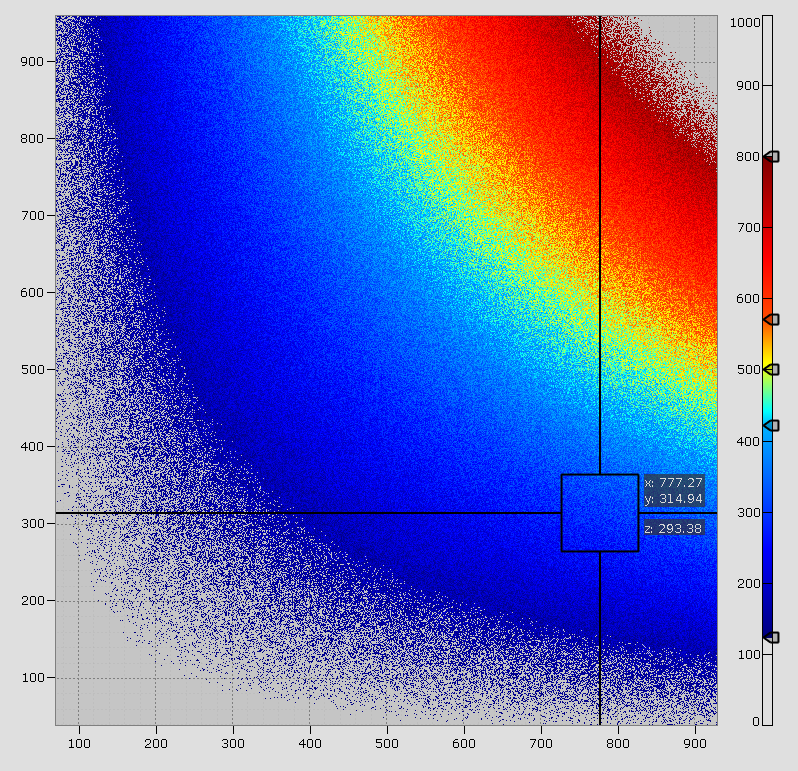
\includegraphics[width=1.0\textwidth]{TaggedHeatMapExample.png}
\caption{Glimpse Heat Map Visualization\cite{glimpse.com}}
\label{heatmap}
\end{figure}

While Glimpse supports basic visual effects using OpenGL shaders, more complicated data analysis is more suited for NVIDIA's Compute Unified Device Architecture\cite{cuda-zone} which exposes GPU hardware for general purpose computation. This project uses CUDA to calculate histograms for subsections of a large heat map in real time and display them using Glimpse visualization tools.

\bibliographystyle{plain}
\bibliography{report}

\end{document}
